\documentclass[letterpaper,12pt]{article}
\usepackage{graphicx}
\usepackage[top=1.10in,right=1.2in,bottom=1.4in,left=1.2in]{geometry} 

\frenchspacing  % Removes extra spacing after period.

\usepackage{hyperref}

\usepackage{natbib}
%\usepackage{times}

\usepackage{amsmath}
%\usepackage{hyperref}

\usepackage{color}

\usepackage{pa}

\newcommand{\proglang}{\texttt}
\newcommand{\pkg}{\texttt}


\title{Ensuring the cross-group comparability of latent variable models for ranking data with the $\da$}

\author{DL Oberski \and JK Vermunt \and GBD Moors}
\date{Department of Methodology and Statistics\\
Tilburg University, The Netherlands}


\usepackage{bm}
\newcommand\vm[1]{% Vector or matrix
\bm{\mathrm{#1}}} 

\newcommand{\av}{\vm{a}}
\newcommand{\vech}{\mathrm{vech}\,}
\newcommand{\vecs}{\mathrm{vec}\,}
\newcommand{\param}{\vm{\theta}}
\newcommand{\bpsi}{\vm{\psi}}
\newcommand{\that}{\hat{\vm{\theta}}}
\newcommand{\psat}{\hat{\vm{\psi}}}
\newcommand{\A}{\vm{A}}
\newcommand{\g}{\vm{g}}
\newcommand{\J}{\vm{J}}
\newcommand{\Id}{\vm{I}}
\newcommand{\Ji}{\vm{J}^{-1}}
\newcommand{\PP}{\vm{P}}
\newcommand{\da}{\textrm{{\sc {EPC}}-interest}}

\usepackage{setspace}
\doublespacing

\begin{document}
\maketitle



\begin{abstract}
Ranking data are often encountered in political science, for example when modeling voters' choices in ``ranked choice'' voting systems or their stated priorities for political goals in a questionnaire. Group comparisons on such measures must first establish whether conclusions of interest are insensitive any differences in measurement--that is, whether the measures are ``equivalent''. To investigate this, the ``$\da$'', a measure of the sensitivity of conclusions to measurement equivalence, was recently introduced in this journal. However, the measure has not been applied to ranking data.

This paper therefore extends the $\da{}$ to the case of latent variable models with ranking data. We demonstrate the approach on a multilevel latent class analysis of three ``(post)materialism'' measures using ranking data from 67,568 respondents in 48 different countries. In this application, violations of measurement equivalence assumptions reverse substantive conclusions of interest; we show that the $\da$ can detect this problem.  

The newly developed methods discussed in this paper have been implemented in user-friendly software for latent variable modeling. Program inputs and data for the examples discussed in this article are provided in the electronic appendix (\url{http://}) [included as zip file in blinded version].
\end{abstract}


\section{Introduction}

\noindent
Ranking  data are central to political science, occurring for example when voters rank candidates in ``ranked choice'' (``instant-runoff'') voting systems such as the Australian federal or London mayoral elections \citep[see e.g][]{karvonen2004preferential,toplak2010preferential},  or when respondents rank objects in a questionnaire, for example  post-materialist value orientations in the World Values Survey \citep{inglehart1997modernization,inglehart2010changing}. 

Such procedures yield categorical and multivariate data, and, since they preclude certain joint outcomes, lead to complex dependencies that must be accounted for. 
Probabilistic models with rankings as outcomes that account for these characteristics were introduced by \citet{thurstone1927law}, and extended by \citet{luce1959individual} and \citet{mcfadden1974conditional}. 

These approaches treat the choices as perfectly measured; however, rankings may contain measurement error, so that latent variable models become necessary. An example can be found in Inglehart's (1997) value scale measuring (post)materialism (see Table \ref{tab:ranking-question}). Respondents are asked to rank their first and second priorities out of four, thus leading to a partial ranking of values priorities. These priorities are divided into ``materialist'' (M in Table \ref{tab:ranking-question}) and ``postmaterialist'' (P) priorities. However, there is error in the measurement of ``postmaterialism'' when using a respondent's ranked priorities. For instance, while valuing a  beautiful countryside  might be a measure of ``postmaterialism'' for, say, a college professor, a farmer depending on ecotourism might prioritize the countryside for more ``materialist'' reasons.  To account for such measurement errors, \citet{croon1989latent} introduced a latent class model for ranking data. \citet{kamakura1994concomitant} extended this model to include covariates relating to class membership. Other approaches to modeling ranking outcomes with latent variables were discussed by \citet{jackson1980factor}, \citet{francis2002analysing} and \citet{maydeu2005structural}.

%\citet{maydeu2005structural} extended \citet{thurstone1927law}'s model to  multivariate outcomes incorporated into a structural equation modeling framework with latent variables \citep[see also][]{brown2011item,brown2012fitting};  \citet{jackson1980factor} described an earlier approach but did not account for the fact that choice data are categorical. \citet{bockenholt2002comparison}  extended \citet{mcfadden1974conditional}'s model to include discrete latent variables with an arbitrary distribution --  ``latent class'' variables. 

% Explain equivalence, EPC-interest

Whenever imperfectly measured variables are to be compared over groups, a concern is whether  such comparisons are ``fair''--that is, whether conclusions about the comparisons of interest are uncontaminated by any differences in measurement across the groups \citep{oberski2012comparability}. For example, Costa Rica's economy depends strongly upon ecotourism, whereas Russia's does not, conceivably causing measurement errors in the item mentioned to differ over these countries. 
%A ``materialist'' inhabitant of Costa Rica, which has no military at all, may not prioritize ``strong defense forces'' as much as an equally ``materialist'' Russian citizen, for instance. In addition, those Costa Ricans whose main source of income is ecotourism might value a ``beautiful countryside'' for entirely ``materialist'' reasons.
%, contrary to citizens of countries in which the countryside is perceived to have a ``postmaterial'' value, but no economic one.  
Such differences may lead a researcher to erroneously conclude that Costa Ricans are less materialist than others. Similarly, when comparing countries with different percentages of women in parliament, the country with the higher percentage\footnote{See Section 2 for data sources.}, Costa Rica (39\%), may erroneously appear to have fewer ``materialists'' than Russia, the country with the lower percentage (14\%). %Some Costa Ricans could, for instance, prioritize the ``postmaterialist'' goal of ``keeping our countryside beautiful'', but for the ``materialist'' reason of promoting ecotourism.
Thus, measurement differences may contaminate conclusions about both mean differences and relationships between variables.

The assumption that groups are comparable in measurement is often called ``measurement equivalence'' or ``measurement invariance'', and evaluating measurement invariance is therefore a concern in any comparative study \citep[see][for reviews]{steenkamp_assessing_1998,vandenberg2000review,schmitt2008measurement}.
%When the results of ranking tasks are compared across countries or other types of groups, not only measurement error, but also ``measurement equivalence''  becomes a concern. Inglehart's ``(post)materialism'' ranking tasks, for example, are often compared across countries to evaluate substantive theories on human values \citep[e.g.][]{inglehart1997modernization}. Such country comparisons may be threatened by cross-country differences in the way respondents' ranking choices measure ``(post)materialism''. In other words, ``measurement equivalence'' means  that conclusions of substantive interest should be uncontaminated by measurement differences \citep{oberski2012comparability}. 
% EPC-interest
Recently, \citet{Oberski:WP:EPC-interest} introduced a measure to evaluate 
measurement invariance in terms of the substantive parameters of interest, the ``EPC-interest''. The researcher initially fits a model that assumes full measurement invariance;  $\da{}$ then estimates the expected change in the parameters of interest that would occur if assumptions of measurement invariance were (partially) relaxed. To continue the previous example, $\da{}$ might indicate how much of the substantive mean difference in  ``materialism'' between Costa Rica and Russia is contaminated by possible measurement differences, and whether this contamination is capable of reversing the conclusions or not. While useful, currently $\da{}$ is only available for linear structural equation models for continuous data. Categorical observed and latent variables are, however, commonly found in the social sciences. Ranking data, moreover, have never been examined for cross-group equivalence in this sense.

This paper therefore develops the $\da{}$ in more generality. This allows for application of the $\da{}$ approach to measurement equivalence evaluation in, for example, IRT models \citep[see also][]{Oberski:WP:model-based-GOF}, ordinal factor analysis, latent class analysis, and to models for ranking data. 
We demonstrate the application of the $\da{}$ to ranking data using comparison of the \citet{inglehart1997modernization} (post)materialism ranking measures over 48 countries. Each country's GDP per capita and percentage of women in parliament is related to the country proportion in categories of ``(post)materialism'' as measured by three separate ranking tasks. Since the measurement of these (post)materialism categories may be flawed,  (post)materialism becomes a latent variable that is discrete: a ``latent class'' variable \citep{bockenholt2002comparison,moors2007heterogeneity}. The measurement model for this variable accounts for the intrinsic dependencies between respondents' ranking choices, while the structural model accounts for dependencies between respondents within a country using a multilevel specification with a nonparametric random effect distribution \citep{vermunt2003multilevel}. The $\da{}$ is then applied to investigate the impact of measurement invariance assumptions on the latent relationship estimates of interest.

%In this study, we apply a recently developed measure for this purpose, the ``EPC-interest'' \citep{Oberski:WP:EPC-interest}, 
%even uitleggen wat dit betekent zou ik zeggen.
%to a  multilevel latent variable model for ranking data.

% Explain LC model (factor analysis with nominal lv), appropriate bc theory is about nominal categories. Multilevel to account for country dependence. Interest on country (between) level covariates. Again appropriate bc of theory. Similar to aggregating to countries  but now account for measurement error and specific ranking process. 
 
%%ik zou de termen nonparametric niet zo prominent gebruiken. Ik zou eerder in de tekst - als je het model beschrijft - ergens  iets latent vallen van dat de verschillen (de random effects) via klassen op groepsniveau ipv normaal verdeelde random effecten. Dus non- of semi-parametrisch. Het model zelf is niet nonparametrisch natuurlijk.
%This ``multilevel latent class'' \citep{vermunt2003multilevel} model for ranks  extends \citet{bockenholt2002comparison}'s model  to include multiple groups and a nonparametric random effect \citep{moors2007heterogeneity}. The  model is applied to 2010 World Values Survey data from 48 countries to evaluate whether country differences in the proportion of latent (post)materialism classes are associated with GDP per capita and percentage of women in a country's parliament, as suggested by values theory. The ``EPC-interest''  measure then approximates the change in these substantive parameters of interest that would be observed if measurement equivalence restrictions were freed. 
%It is therefore a sensitivity analysis approach to measurement equivalence \citep{Oberski:WP:EPC-interest}; moreover, \citet[p. 12]{schoot2013facing} argued that it can be seen  as providing a specific definition of ``approximate'' measurement equivalence \citep[see][for other approaches]{muthen2012bayesian,muthen2014alignment}.
%Since the EPC-interest was originally developed for the case of equality restrictions in linear structural equation models with continuous data, we extend the EPC-interest measure here to include categorical observed and latent variables. 

% Change to methodological contribution
%The contributions of this paper are threefold. First, contrary to existing uses of these data, we allow for measurement error in the (post)materialism ranking tasks. Moreover, no assumptions about the distribution of these errors or the underlying scale are necessary. Second, we evaluate whether the 48 countries in the 2010 World Values Survey can be compared for the purpose of looking at the relationship between (post)materialism and correlates central to \citet{inglehart1997modernization}'s theory. Third, we develop the EPC-interest measure for latent class analysis, i.e. for models with discrete observed and latent variables. 
%This development allows for more general application of the EPC-interest approach to measurement equivalence evaluation, for example in IRT analysis \citep[see also][]{Oberski:WP:model-based-GOF} or ordinal factor analysis. 

\bigskip

% Change to methodological contribution
Section \ref{sec:data} presents the data and the postmaterialism theory used in the example application model. Since the obtained measures are rankings, Section \ref{sec:model} then presents the multilevel latent class model for partial rankings. We then present the EPC-interest for such and other latent variable models in Section \ref{sec:epc-interest}, after which the results of applying the EPC-interest to the postmaterialism model and data is discussed in Section \ref{sec:results}. Finally, Section \ref{sec:discussion} provides some conclusions and discusses limitations and further connections with other work.


\section{Background and Data for example application}

\begin{table}
\label{sec:data}
\caption{\label{tab:ranking-question}
Value priorities to be ranked for the three WVS 2010--2012 ranking sets. ``Materialist'' concerns are marked ``M'' while ``postmaterialist'' concerns are marked ``P''.
The wording is ``People sometimes talk about what the aims of this country should be for the next ten years. On this card are listed some of the goals which different people would give top priority. Would you please say which one of these you, yourself, consider the most important?''; ``And which would be the next most important?''.
}
\begin{tabular}{p{0.01\textwidth}rrp{0.72\textwidth}}
\hline
& Option \# &M/P& Value wording\\
\hline
\multicolumn{3}{l}{\emph{Set A}}\\
&1. & M &A high level of economic growth\\
&2. & M &Making sure this country has strong defense forces \\
&3. & P &Seeing that people have more say about how things are done at their jobs and in their communities\\
&4. & P &Trying to make our cities and countryside more beautiful\\

\multicolumn{3}{l}{\emph{Set B}}\\
&1. & M &	Maintaining order in the nation\\
&2. & P &Giving people more say in important government decisions \\
&3. & M &	Fighting rising prices\\
&4. & P &Protecting freedom of speech\\

\multicolumn{3}{l}{\emph{Set C}}\\
&1. & M &	A stable economy\\
&2. & P &Progress toward a less impersonal and more humane society \\
&3. & P &	Progress toward a society in which ideas count more than money \\
&4. & M &	The fight against crime\\
\hline
	\end{tabular}
\end{table}


Our example application employs the 2010--2012 World Values Survey\footnote{\url{http://www.worldvaluessurvey.org/}} (WVS) comprising $n = 67,568$ respondents in 48 different countries (Appendix \ref{sec:countries-included} provides a full list of countries).
The WVS questionnaire includes \citet{inglehart1977silent}'s extended (post)materialism questions, developed to measure political values priorities. This extended version includes three sets of four priorities (Table \ref{tab:ranking-question}). Of these, set B in Table \ref{tab:ranking-question} is known as the ``short scale'' that is commonly used in research on values priorities.  
%Two of the values in each set are intended to measure  ``materialist'' concerns while the two remaining priorities indicate ``postmaterialist'' political goals; for each of the   three sets, WVS respondents are then asked to select their first and second priorities. 
%Thus, this procedure yields an incomplete (partial) ranking: only first choice and second choice are known, while the  rank order is unknown for the remaining two objects.



%Inglehart labels the latter goals as post-materialist to indicate that the priority of these goals increases when materialist goals are established and hence drop in priority level in the given set. 

(Post)materialism theory is based on the ``dual-hypotheses model'' \citep[p. 881]{inglehart1981post}. The first hypothesis holds that an individual's priority set reflects the socio-economic environment because one attaches relatively more importance to scarce objects. In line with this scarcity hypothesis, \citet{inglehart1997modernization} and \citet{inglehart2010changing} argued that socio-economic development indicators per country such as GDP per capita will correlate strongly with aggregated values scores. 

The second, ``socialization'', hypothesis stresses the importance of experiences in the ``formative'' years. By a process of social metabolism, society gradually changes from  materialist to postmaterialist.
In line with the socialization hypothesis, associations of aggregated values priorities with socio-cultural variations across countries such as religious heritage and gender equality have been predicted and found by \citet{inglehart2002gender}. 

%The latter hypothesis constitutes the heart of the argument regarding generational differences in political priorities since it indicates that, in reaching adulthood, values tend to crystallize in personality. By a process of social metabolism, society gradually changes from  materialist to postmaterialist. %The socialization hypothesis is crucial in understanding generational differences. The socio-economic proposition on the other hand gains momentum when comparing different cultures. 
%Moreover, in line with the socialization hypothesis, 
In short, substantive interest in this literature focuses on the associations between (post)materialism and both socio-economic and socio-cultural country-level aggregates. 
We will follow these authors and examine the aggregate relationship of values priorities with log-GDP per capita and the percentage of women in parliament. 
These country-level variables were obtained from the World Bank database\footnote{\url{http://data.worldbank.org/}} using the \texttt{WDI} package \citep{arel2013WDI} in \texttt{R 3.0.2} \citep{Rlanguage}.


%In their previous work, Inglehart and colleagues examined these relationships of interest between value priorities and country-level covariates by creating an observed categorization of the ranking choices into three groups:  ``materialist'', ``postmaterialist'', and ``mixed''. These groups are determined by whether the first and second choice on the second ranking set are both ``materialist'', ``postmaterialist'', or a combination of the two.  Thus, these groups are defined \emph{a priori}, and their usage as observed variables implies that a complete absence of measurement error is assumed.  This assumption can be questioned since \citet{clarke1999effect} demonstrated that the rating versions of (post)materialism measures contain considerable nuisance variability. It also implies that no differences in measurement exist across the countries to be compared \citep{ippel2014investigating}. In other words, any comparison of the created categories over countries is assumed to be fully due to substantive rather than measurement differences. The contribution of  this study to the values priorities literature is to relax the assumption of zero measurement error, examine empirically whether three classes can adequately represent the data, and apply the EPC-interest procedure to examine the implicit claim of full cross-country equivalence of these measures. 




\section{Model}
\label{sec:model}

%In feite gebruiken we gewoon het model van Kamakura, Wedel en Agrawal, wat een uitbreiding is naar covariaten en attributen van het model van Croon. Je kunt het ook zien als een uitbreiding naar klassen van het rankorder of exploded logit model.
To examine differences in (post)materialism with respect to GDP per capita and the proportion of women in parliament, we develop a latent variable model for ranking data. The advantages of this approach are that there is no need to establish a priori rules for combining the three ranking tasks into a measure of ``(post)materialism''; that it does not presuppose a fixed number of ``(post)materialism'' classes; that it allows for measurement error in ``(post)materialism''; and that it allows for an examination of the impact of violations of measurement invariance on the conclusions of interest. 

In each of the $C$ countries we observe $\{n_1,\ldots, n_C\}$ respondents. Each respondent $i$ has ranked their first and second choice on three ranking tasks A, B, and C (see Table \ref{tab:ranking-question}); that is, only first choice and second choice are known. We assume that each object (e.g. value priority) has a particular ``utility'' and that the probability of choosing an object for each rank is proportional to that utility \citep[p. 171]{luce1959individual,bockenholt2002comparison}. Following \citet{croon1989latent} and \citet[p. 172]{bockenholt2002comparison}, we then model the probability of these rankings conditionally on unit $i$'s membership of latent class variable $X$, so that object utilities can differ over respondents in different classes. This latent class variable $X$ in our case will represent ``(post)materialism''. For example, for ranking task $A$ in country $c$, respondent $i$'s  choices for first and second place are modeled as
 \begin{equation}
	P(A_{1ic} = a_1, A_{2ic} = a_2 | X_{ic} = x) = 
		\frac{\omega_{a_1 x}}{\sum_{k} \omega_{k x}}
		\frac{\omega_{a_2 x}}{\sum_{k \neq a_1}
			\omega_{k x}},
				\label{eq:ranking}
\end{equation}
where $\omega_{k x}$ is the ``utility'' of object $k$ for respondents in class $x$. Crucially, the choice for second place, $A_{2ic}$, is modeled while excluding the alternative already chosen for first place, $A_{1ic}$. In other words, we model a sequential ranking process in which first place is chosen from all options, then second place is chosen from the remaining options.
This dependency intrinsic to ranking tasks makes the model used here different from standard models for qualitative dependent variables  such as multinomial regression.
%such as latent class or ordinal factor analysis models.

To facilitate model interpretation, it is convenient to separate the class-specific utilities into log-linear intercept $\tau_{k}$ and slope $ \lambda_{k x}$,
\begin{equation}
	\ln \omega_{k x} = \tau_{k} + \lambda_{k x}.\label{eq:loglin-measurement}
\end{equation}
For identification, we use the ``effects coding'' \citep{vermunt2013technical} sum-to-zero restrictions $\sum_k \tau_{k} = \sum_{k} \lambda_{kx} = \sum_{x} \lambda_{kx} = 0$. The attribute parameters $\lambda_{k x}$ can then be interpreted as the deviation from option $k$'s average log-utility in latent class $x$. % $9 (T - 1)$ 

Primary interest focuses on how the probabilities of belonging to these latent (post)materialism classes differ as a function of the country-level covariates log-GDP per capita ($Z_1$) and percentage of women in parliament ($Z_2$).  At the same time, it has become common practice to control for dependencies between units in the same country using a multilevel approach. We therefore model the probability that unit $i$ in country $c$ belongs to latent class $x$ using the multilevel multinomial logistic regression
\begin{equation}
P(X_{ic} = x| Z_{1ic} = z_{1ic}, Z_{2ic} = z_2, G_c = g) = \frac{\exp(\alpha_x + \gamma_{1x} z_1 +\gamma_{2x} z_2  + \beta_{gx})}
					{\sum_t \exp(\alpha_t + \gamma_{1t} z_1 +  \gamma_{2t} z_2 +  + \beta_{tg})},
					\label{eq:regression}
\end{equation}
where the country-level random effect variable $G$ has been introduced. The random effects $\beta_{tx}$ in Equation \ref{eq:regression} could be assumed to have a Gaussian (normal) distribution, leading to a standard multilevel model. However,  in the past very differing classes of countries have been observed \citep{vermunt2003multilevel}, 
%Wij hebben geen multilevel LC model gebruikt. We hebben wel gekeken naar landen verschillen, en die komen erop neer dat deze landen beter kunnen worden geclusterd dan ze te laten vari�ren op een onderliggende continue variabele. Overigens past dit clustereren ook goed bij hoe hier inhoudelijk naar wordt gekeken. Ik mijn  2003 paper heb ik wel multilevel LC toegepast, maar dan enkel op item B.
so that the normality assumption is rather implausible. Since an incorrect parametric specification of the distribution of $G$ can bias the results \citep[e.g.][p. 275]{heckman1984method}, we instead take $G$ to be a country-level latent class variable with $S$ classes and a freely estimated (nonparametric) distribution. Overall, then, our model can be seen as a multilevel multinomial regression of (post)materialism on country-level covariates, in which the nominal dependent variable is latent (corrected for misclassification), and the random effects distribution is nonparametric rather than Gaussian.  
%Beschouw je de clustering van landen gewoon als een soort noise, als een handige/niet-parametrische manier om met niet verklaarde verschillen tussen landen om te gaan? Dat zou ik dan expliciet zeggen. De volgende zin volg dan automatisch: de effecten van GDP en %Women zijn de parameters of interest.
The main parameters of substantive interest in Equation \ref{eq:regression} are therefore the multinomial logistic regression coefficients $\gamma_{mx}$. 


%, of which there are $2  (T - 1)$, where $T$ is the number of latent postmaterialism ($X$) classes. 
%It may also be of interest to derive the posterior probability for each country, $P(X | \text{country}) = \sum_{i \in \text{country}} P(Y | X) P(X) / \sum_X P(Y | X)$ for visual display purposes.

Combining the three ranking tasks, each modeled according to Equation \ref{eq:ranking}, with the multilevel latent class regression model in Equation \ref{eq:regression} leads to the full data likelihood
%Je hebt geen casewise maar een groupwise likelihood. De casewise likelihood, heb je enkel conditioneel op G. Sommeren over G doe je pas na vermenigvuldigen over alle cases binnen een groep.
\begin{multline}
L(\param) = 
	P(A_1, A_2, 
		B_1, B_2, 
		C_1, C_2 | Z_1, Z_2) = \\
	\prod_{c = 1}^{C}
	\sum_{G} P(G_c)	
	\prod_{i = 1}^{n_c}
	\sum_{X} P(X_{ic} | Z_{1ic}, Z_{2ic}, G_c) \times\\
				P(A_{1ic}, A_{2ic} | X_{ic})
				P(B_{1ic}, B_{2ic} | X_{ic}) 
				P(C_{1ic}, C_{2ic} | X_{ic}),
				\label{eq:lik}
\end{multline}
where the realizations of variables have been dropped for clarity, and $\param$ is a vector collecting the free parameters of the model\footnote{There are $ T (11 + S) -3$ free parameters overall.}. 
%Note that values of the within-country variables $X, A_1, A_2, B_1, B_2, C_1$, and $C_2$ may differ over persons, whereas the between-country variables $G, Z_1$, and $Z_2$ can differ only over countries. 
To obtain the likelihood in Equation \ref{eq:lik},  $G$ is assumed to fully account for the dependency between units within countries, and $X$ fully accounts for the dependency between units within a country, i.e.  units are i.i.d. given $X$, and country likelihoods are independent given $G$. 


\begin{figure}\centering
	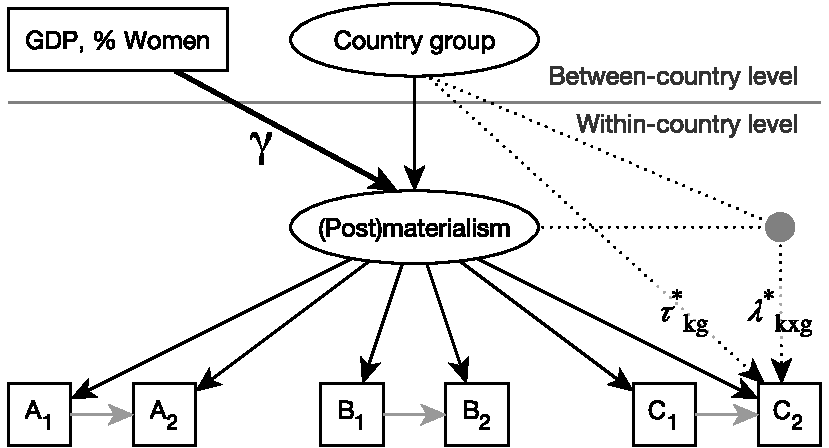
\includegraphics[width=0.7\textwidth]{figures/model}
	\caption{\label{fig:model}Graphical representation of 
	the multilevel latent class regression model for 
	(post)materialism measured by three partial ranking tasks. Observed variables are shown in rectangles while unobserved (``latent'') variables are shown in ellipses.	}
\end{figure}


Figure \ref{fig:model} shows a graphical representation of the model in Equation \ref{eq:lik}. 
The parameters of primary substantive interest are the effect-coded logistic regression coefficients for the effect of GDP per capita and percentage of women in parliament on the latent postmaterialism class (the stronger line labeled $\gamma$ in Figure \ref{fig:model}). 
%These effects of interest are controlled for the country random effects. 
The top part of the model in Figure \ref{fig:model} is a multilevel latent class regression. The gray arrows between indicators within the same set are meant to show that a fixed conditional relationship is specified between the first and second choice within each set (Equation \ref{eq:ranking}). 

Equation \ref{eq:lik} is, in fact, a ``full measurement invariance'' model: the measurement of (post)materialism by the three ranking tasks is  not allowed to differ over countries. 
This excludes potential violations of ``scalar''  and ``metric'' measurement invariance, which can be conceptualized as, respectively, a direct main effect and a direct interaction effect of the grouping variable 
\citep{mellenbergh1989item,kankaras2010testing,kankaras2011measurement}. Since we do not employ multiple groups (fixed effects) to deal with country effects, but a latent class multilevel (random effects) approach, instead of considering main and interaction effects from the countries directly, we consider these for the country random effects ($G$)  \citep[see][]{dejong2007relaxing,fox2011random,verhagen2013bayesian,jak2013test,jak2014measurement}.
Thus, measurement invariance violations could be parameterized by extending Equation  \ref{eq:loglin-measurement} to include country group class ($g$) effects:
\begin{equation}
	\ln \omega_{k x g} = \tau_{k} + \lambda_{k x} + 
		\tau^{*}_{k g} + \lambda^{*}_{k x g}.
			\label{eq:loglin-measurement-noninvariant}
\end{equation}
The base invariance model above can then be seen as fixing the intercept deviations $\tau^{*}_{k g}$  and slope deviations $\lambda^{*}_{k x g}$ to 0.  An example of this parameterization of measurement non-invariance for 
the second ranking of Set C ($C_2$) is shown in Figure \ref{fig:model} as the dotted main effect and interaction effects for scalar and metric invariance, respectively. 

With three sets of three non-redundant priorities each, there are $9 (S - 1) T$ possible additional $\tau^{*}_{k g}$ and $\lambda^{*}_{k x g}$ parameters representing misspecification in the full invariance model specified above. For example, with $S=3, T=3$, there will be $54$ possible violations of invariance. %With three or more second-level classes ($S \geq 3$), there are more possible violations of measurement invariance than there are parameters in the base model.
This is clearly a very large number of potential violations of measurement invariance, with an astronomical ($\approx 1.8 \times 10^{16}$) number of possible subsets of non-invariant models, making the fitting of each of these possible submodels infeasible. The EPC-interest, which considers the possible effect of freeing each of the restrictions separately, is therefore an attractive alternative. 

However, there are strong dependencies between the additional parameter estimates. First, estimates of parameters corresponding to  different categories of the same variable will necessarily be strongly dependent. Second, parameters corresponding to the same ranking set (A, B, or C) will be highly dependent due to the necessary dependence between the first and second choice in a ranking task. Therefore, instead of considering only one possible misspecification at a time, we consider freeing sets of restrictions corresponding to all main effects and all interaction effects of each set. The advantages are that the estimated change in the parameters of interest will be closer to the observed change when freeing these restrictions, and that a model space to be explored of order $10^{16}$ is reduced to the examination of the effect of six sets of misspecifications on $2 (T-1)$  parameters of interest, $\gamma_{jx}$.

\bigskip
In summary, we have attacked the problem of examining the differences in (post)-materialism over 48 countries with different levels of GDP per capita and percentage of women in parliament by formulating a multilevel latent class model for ranking data. Measurement invariance is important here because direct main and interaction effects from country groups on the ranking tasks could threaten the comparison of countries with different levels of the covariates. Therefore it becomes relevant to examine the impact of these possible violations of measurement invariance on the parameters of substantive interest. The following section will introduce a method for doing so without the need to fit the alternative models. 


\section{EPC-interest}
\label{sec:epc-interest}

In the application discussed, as in any application of invariance testing, interest focuses on a particular (function of) free parameters of the model. As argued by \citet{oberski2012comparability,Oberski:WP:EPC-interest}, the question of invariance testing is then relevant insofar as it affects these parameters of interest. Such parameters may differ in models that allow for non-invariance, which in the model introduced in the previous section was parameterized as direct main and interaction effects of a group random effect. Instead of investigating whether such effects are statistically significantly different from zero, we suggest to investigate the impact of such effects on the parameters of interest. This  is done using the ``expected parameter change'' in the parameter of interest, ``$\da$''.

The ``$\da$'' estimates the change in a free parameter of the model that one can expect to observe if a particular restriction were freed. It is therefore a method of sensitivity analysis. However, the researcher is not forced to estimate all possible alternative models, but can evaluate the sensitivity of the results after fitting the restrictive full invariance model. 
The $\da{}$ is based on the work of \citet{saris_detection_1987}, who introduced the expected parameter change in a fixed parameter for linear structural equation models (SEM), and \citet{bentler1993some}, who introduced the expected parameter change in a free parameter after freeing a fixed parameter for SEM. \citet{Oberski:WP:EPC-interest} suggested using the $\da{}$ for invariance testing using linear structural equation models with continuous data.

In this section we develop the $\da{}$ in some generality so as to be useful for a larger set of models than just that applied in the example. In principle EPC-interest developed below applies to any situation in which parameters of interest are estimated by maximum likelihood and the researcher wishes to consider the likely effect on the parameters of interest that freeing some nuisance parameter might have. This is particularly useful for the case of latent variable modeling, in which the parameters of interest are typically the structural parameters (e.g. regression coefficients between latent variables) and the nuisance parameters are often measurement parameters. In the special case of invariance testing, the nuisance parameters can be conceived of as direct main and interaction effects of group dummy variables or random effects, or, equivalently, as differences between groups in measurement parameters.

We also extend the $\da$ to evaluate the probable impact of several misspecifications at the same time. This last extension is particularly relevant in categorical data models, since parameters related to different categories of the same variable are often highly dependent. In such cases, the impact of misspecifications is better evaluated in sets of strongly related parameters. In the application to ranking data discussed above, for instance, parameters relating to the different ranking objects in the same set will be highly dependent, since the second choice in each ranking is modeled conditionally upon the first choice (Equation \ref{eq:ranking}). The impact of freeing the parameter $\lambda_{111}$ can therefore not be seen separately from that of $\lambda_{211}, \lambda_{121}$, etc. We therefore consider the impact of all possible interactions of country grouping $G$ with the latent (post)materialism variable $X$ jointly for each of the three ranking tasks. 

The key concept is considering the likelihood not only as a function of the free parameters of the model, but also as a function of the parameters that are fixed to obtain the full invariance model. Collecting the free parameters in a vector $\param$ and the fixed parameters in a vector $\bpsi$, we assume the likelihood can be written as an explicit function of both sets of parameters, $L(\param, \bpsi)$.  The maximum-likelihood estimates $\that$ of the free parameters can then be seen as obtained under the full invariance model that sets $\bpsi=0$, i.e. $\that = \arg\max_{\param} L(\param, \bpsi = 0)$. Further, define the parameters of substantive interest as $\vm{\pi} := \vm{P} \param$, where $\vm{P}$ is typically a logical (0/1) selection matrix, although any linear function of the free parameters $\param$ may be taken. 
Interest then focuses on the likely value these free parameters $\vm{\pi}$ would take if the fixed $\bpsi$ parameters were freed in an alternative model, $\hat{\vm{\pi}}_a = \vm{P} \arg\max_{\param, \bpsi} L(\param, \bpsi)$. 

We now show how these changes in the parameters of interest as a consequence of freeing the fixed parameters $\bpsi$ can be estimated without fitting the alternative model. Let the Hessian $\hat{\vm{H}}_{\vm{a}\vm{b}}$ be the matrix of second derivatives of the likelihood with respect to vectors $\vm{a}$ and $\vm{b}$, evaluated at the maximum likelihood solution of the full invariance model, $\hat{\vm{H}}_{\vm{a}\vm{b}} := (\partial^2 L /\partial \vm{a} \partial \vm{b}^\prime)|_{\param=\that}$. 
The expected change in the parameters of interest is then measured by the $\da$, 
\begin{equation}
\da = \hat{\vm{\pi}}_a - \hat{\vm{\pi}} = \vm{P}
%	\left( \frac{\partial^2 L(\param, \bpsi)}{\partial (\param, \bpsi)^\prime \partial (\param, \bpsi)} \right)^{-1}
%		\vm{D}^{-1} \hat{\vm{H}}_{\param\bpsi}^\prime \hat{\vm{H}}^{-1}_{\param\param}
\hat{\vm{H}}^{-1}_{\param\param} \hat{\vm{H}}_{\param\bpsi}\vm{D}^{-1}
		\left[ \left.\frac{\partial L(\param, \bpsi)}{\partial \bpsi}\right|_{\param = \that} \right] +	
		O(\vm{\delta}^\prime\vm{\delta}),
		\label{eq:epc-interest}
\end{equation}
where $\vm{D}:= \hat{\vm{H}}_{\bpsi\bpsi} - \hat{\vm{H}}_{\param\bpsi}^\prime \hat{\vm{H}}^{-1}_{\param\param} \hat{\vm{H}}_{\param\bpsi}$ and the deviation from the true values is $\vm{\delta}:= \vm{\vartheta} - \hat{\vm{\vartheta}}$, with $\vm{\vartheta}$ collecting the free and fixed parameters in a vector, $\vm{\vartheta}:= (\param^\prime, \bpsi^\prime)^\prime$. Note that, apart from the order of approximation term $O(\vm{\delta}^\prime \vm{\delta})$,  Equation \ref{eq:epc-interest} contains only terms that can be calculated after fitting the invariance model.
%(Relevant derivatives for the special case of the multilevel latent class model are given in Appendix \ref{app:derivatives}.)
 Thus, it is not necessary to fit the alternative model to obtain the $\da{}$.

In the structural equation modeling literature, the expected change in the fixed parameters $\bpsi$  is commonly found and implemented in standard SEM software. This measure is commonly know as the ``EPC'', but to avoid confusion we term it ``EPC-self'' here. The EPC-self and $\da{}$ both consider the impact of freeing restrictions, but differ in the target of this impact: the EPC-self evaluates the impact on the restriction itself, whereas the $\da{}$ evaluates the impact on the parameters of interest. In spite of these differences, the two measures are related: this can be seen by recognizing that $- \vm{D}^{-1}
		\left[ \left.\frac{\partial L(\param, \bpsi)}{\partial \bpsi}\right|_{\param = \that} \right] = \text{EPC-self} \approx \bpsi - \hat{\bpsi}$ so that, from Equation \ref{eq:epc-interest}, 
\begin{equation}
\da=- \vm{P} \hat{\vm{H}}^{-1}_{\param\param} \hat{\vm{H}}_{\param\bpsi} \,\text{EPC-self} \approx
- \vm{P} \hat{\vm{H}}^{-1}_{\param\param} \hat{\vm{H}}_{\param\bpsi} \left( \bpsi - \hat{\bpsi}\right)
\end{equation}
Furthermore, since $\hat{\bpsi}$ and $\hat{\param}$ are implicitly related by the fact that they are both solutions to the equation $\partial L / \partial \vm\vartheta = \vm{0}$, invoking the implicit function theorem yields $- \hat{\vm{H}}^{-1}_{\param\param} \hat{\vm{H}}_{\param\bpsi}  = \partial \param / \partial \bpsi^\prime$, so that 
\begin{equation}
	\da = \vm{P} \left( \frac{\partial \param} {\partial \bpsi^\prime} \right) \left( \bpsi - \hat{\bpsi}\right),
	\label{eq:epc-linear}
\end{equation}
that is, the $\da{}$ can be seen simply as the coefficient of a linear approximation to the relationship between the free and fixed parameters, multiplied by the change in the fixed parameters. This demonstrates the difference with the sensitivity analysis approach common in econometrics \citep[p. 168]{magnus2007local} and applied to SEM by \citet{yuan2003assessing}, in which only $\partial \param / \partial \bpsi^\prime$ is considered: the $\da{}$ combines both the direction ($\partial \param / \partial \bpsi^\prime$) and the magnitude ($ \bpsi - \hat{\bpsi}$) of the misspecification.


The derivation of the $\da{}$ given in Equation \ref{eq:epc-interest} starts from the full invariance solution. We then find a hypothetical new  maximum of the likelihood by setting the gradient of a Taylor expansion of the likelihood around the full invariance solution to zero:
\begin{equation}
 \frac{\partial L(\param, \bpsi)}{\partial \vm{\vartheta}}= \vm{0} = 
	\left( \begin{array}{cc}
	\frac{\partial L(\param, \bpsi) }{ \partial \param}|_{\param=\that}\\
	\frac{\partial L(\param, \bpsi) }{ \partial \bpsi}|_{\param=\that}\\
	\end{array} \right)  + 
%	\left(\frac{\partial^2 L(\param, \bpsi) }{ \partial \vm{\vartheta}^\prime \partial \vm{\vartheta}} \right)
	\left( \begin{array}{cc}
		\hat{\vm{H}}_{\param\param} & \hat{\vm{H}}_{\bpsi\param}\\
		\hat{\vm{H}}_{\bpsi\param} & \hat{\vm{H}}_{\bpsi\bpsi}\\
	\end{array} \right)  
		\left( \begin{array}{cc}
		\param - \that\\
		\bpsi - \hat{\bpsi}
	\end{array} \right)+
O(\vm{\delta}^\prime\vm{\delta}).
	\label{eq:gradient}
\end{equation}
A similar device was used to derive the so-called ``modification index'' or ``score test'' for the significance of the hypothesis $\bpsi = \vm{0}$ by \citet[p. 373]{sorbom1989model}.
Equation \ref{eq:epc-interest}  follows directly by noting that $( \partial L(\param, \bpsi) / \partial \param ) |_{\param=\that} = \vm{0}$ and applying the standard linear algebra result on the inverse of a partitioned matrix $\left(\hat{\vm{H}}^{-1}\right)_{\param\bpsi} = 	- \hat{\vm{H}}^{-1}_{\param\param} \hat{\vm{H}}_{\param\bpsi}\vm{D}^{-1}$ \citep[e.g.][p. 12]{magnus2007matrix}.

The accuracy of the approximation of the $\da{}$ as a measure of the change in the parameters of interest is reflected in the order of approximation term, $O(\vm{\delta}^\prime\vm{\delta})$. It can be seen that this accuracy is quadratic in the overall change in parameters, so that the approximation can be expected to work best when the misspecifications are not ``too large''. This result corresponds to results on the score test (``modification index'') and ``EPC-self'' in the literature on structural equation modeling, which can be shown to be exact under a ``sequence of local alternatives'', i.e. when $\vm{\vartheta} = \lim_{n\rightarrow\infty} \hat{\vm{\vartheta}} + n^{-\frac{1}{2}}\vm{\delta}$ \citep[p. 135]{satorra1989alternative}.
It is important to note here that $\vm{\delta}$ is the deviation from the ``true'' value of $\vm{\vartheta}$, rather than the deviation from the limit of the parameter estimates under the alternative model. Therefore another view on the accuracy is that it will be better when the alternative model is not strongly misspecified. For this reason it is also important to consider freeing sets of very strongly related parameters simultaneously, since a change in one of them will then imply a change in the others, and, consequently, a misspecified alternative model.

%Applying standard theory of variance estimation in misspecified models \citep{white1982maximum}, this second-order term suggests that the variance of $\da{}$ can be estimated as
%\begin{equation}
%	\widehat{\text{avar}}(\da) = \vm{P} 		\vm{D}^{-1} \hat{\vm{H}}_{\param\bpsi}^\prime \hat{\vm{H}}^{-1}_{\param\param} 
%	\hat{\vm{B}}_{\bpsi\bpsi}
%\hat{\vm{H}}^{-1}_{\param\param} \hat{\vm{H}}_{\param\bpsi}	\vm{D}^{-1} \vm{P}^\prime,
%\end{equation}
%where $\hat{\vm{B}}_{\bpsi\bpsi}$ is the outer product matrix evaluated at the MLE. 

%The Hessian matrix $\vm{H}$ 


\section{Results}
\label{sec:results}


We now estimate the multilevel latent class model using 48 countries from the World Values Survey\footnote{\url{http://www.worldvaluessurvey.org}} for  2010--2012. Since our goal is to compare countries with different levels of GDP per capita and proportion of women in parliament, in this study we evaluate the sensitivity of these effect estimates of interest to measurement invariance assumptions using the $\da$.

The model as well as $\da{}$ measures  were implemented by one of the authors in the software Latent Gold Choice version 5.0.0.14157 and higher \citep[pp. 135--136]{vermunt2005lgchoice,vermunt2013technical}. Program input for this analysis can be found in Appendix \ref{sec:LGinput}, while output and data are included in the online Appendix at \url{http://[BLINDED]}.


We select three  classes for both the latent ``(post)materialism'' variable and the country group class variable. For BIC values and the rationale behind these choices, please see Appendix \ref{app:bic}. Since class selection is not the focus of this example analysis, we will not discuss it here further. 

The full invariance model imposes $\tau^*_{jkg} = 0$ and $\lambda^*_{jkxg} = 0$, i.e. there is no difference in measurement over the group random effect variable. Such violations of measurement invariance are relevant in the present analysis because they could potentially threaten the conclusions of substantive interest, namely the relationships $\gamma$ between (post)materialism on the one hand and GDP per capita and percentage of women in parliament on the other. In this particular analysis, it was thought to be pertinent whether, after freeing some of the measurement invariance restrictions,  one of these regression coefficients of interest could be estimated with a reversed sign. 

We therefore calculated the $\da{}$ for these parameters, of which our three-class model has four: two for each for each of the two independent variables. Measurement invariance violations can potentially take the form of 6 direct main effects ($\tau^{*}_{j k g}$) --$(4-1)$ category effects in $(3-1)$ classes--  and 12 direct interaction effects ($\lambda^{*}_{j k x g}$) for each of the three ranking tasks, totaling 54 possible misspecifications in the full invariance model. However, these misspecifications are strongly correlated and should not be considered separately. Rather, we consider the probable impact on the $\gamma$ parameters of interest of freeing the direct main effects for each ranking task separately and of freeing the  direct interactions for each ranking task separately. In short, rather than consider the direct and interaction effects for each of the 48 countries on each of the 3 unique categories of each of the three ranking tasks, making for $4 \times 3 \times (4 - 1)\times  (48 - 1) \times(1 + (3 - 1)) = 5076$ potential $\da{}$ values, we evaluate direct effects of the country group random effect and consider their impact jointly for strongly correlated misspecifications, reducing the problem to 24 $\da{}$ values of interest.


\begin{table}
	\caption{Full invariance multilevel latent class model: parameter estimates of interest with standard errors (columns 3 and 4), as well as expected change in these parameters measured by the  $\da{}$ when freeing each of six sets of possible misspecifications (columns 5--10). \label{tab:epc-interest-model1}}
	\begin{tabular}{lrrrrrrrrrrr}
	\hline
		&&&&&\multicolumn{7}{c}{EPC-interest for...}\\
	&&&&&\multicolumn{3}{c}{$\tau^{*}_{j k g}$} && \multicolumn{3}{c}{$\lambda^{*}_{j k x g}$}\\
			\hline
		&&\multicolumn{2}{c}{Estimates}&&\multicolumn{3}{c}{Ranking task} && \multicolumn{3}{c}{Ranking task}\\
\cline{3-4}\cline{6-8}\cline{10-12}
			&	&	Est.&	s.e.&	&	1  &	2  &	3  &&	  1&	2 &	3\\
				\hline
Class	1&	GDP&	-0.035&	(0.007)&	&	-0.013&	0.021&	-0.002&&	\textbf{0.073}&	\textbf{0.252}&	0.005\\
Class	2&	GDP&	-0.198&	(0.012)&	&	-0.018&	-0.035&	0.015&&	-0.163&	-0.058&	0.002\\
\\
Class	1&	Women&	0.013&	(0.001)&	&	-0.006&	0.002&	0.000&&	-0.003&	0.029&	0.002\\
Class	2&	Women&	-0.037&	(0.001)&	&	0.007&	-0.003&	0.002&&	-0.006&	-0.013&	0.002\\
	\hline
\end{tabular}
\end{table}

Table \ref{tab:epc-interest-model1} shows these 34 $\da{}$ values calculated from the full invariance model. These $\da{}$ values estimate the likely change from the maximum likelihood estimates (column 3 in Table \ref{tab:epc-interest-model1}) in the four parameters of substantive interest after freeing the direct main or interaction effects for each of the three ranking tasks (columns 5--10 in  Table \ref{tab:epc-interest-model1}). In the full invariance model, Class 1 corresponds to a ``postmaterialism'' class. The estimate -0.035 (s.e. 0.007) shown in Table \ref{tab:epc-interest-model1}) would therefore suggest that more prosperous nations tend to be less postmaterialist. This directly contradicts the theory of \citet{inglehart1997modernization}, which suggests that this coefficient should be positive. 

Since the theory specifies only that certain coefficients should be positive or negative, the key focus of substantive interest should be whether misspecifications in the invariance model can potentially change the sign of a parameter of interest. In Table \ref{tab:epc-interest-model1}, we therefore look for $\da{}$ values that, when added to the estimates in column 3, would change the sign of those estimates. It can be seen in the Table that two such $\da{}$ are indeed present, namely the direct interaction effect of the country group class with the postmaterialism class on ranking tasks 1 and 2. The analogous finding \citep{kankaras2011measurement} if CFA had been used would be that of ``metric equivalence'' for ranking task 3 but not ranking tasks 1 and 2.  This means that the attribute parameters that define the classes for these two tasks differ over country groups, and that after accounting for these differences the effect of GDP on postmaterialism is estimated to be positive rather than negative. This set of misspecifications is thus of substantive interest and should be amended in the model. 

We therefore free these two sets of measurement invariance violations, allowing for differences in the parameters of ranking tasks 1 and 2 across country groups. Table \ref{tab:epc-interest-model2} shows the substantive parameter estimates and $\da{}$ interest values for the resulting partial invariance model, which has 63 parameters and a log-likelihood of $-418610.0$ ($\text{BIC} = 837920.5$). The likelihood ratio test of improvement in model fit is highly significant ($\chi^2_{\text{df} = 28} = 24607$). Moreover, the substantive logistic regression coefficient for the effect of GDP on the postmaterialism class (Class 2 in Table \ref{tab:epc-interest-model2}), is indeed positive after freeing the detected misspecifications. Re-calculating $\da{}$ values for the remaining possible misspecifications reveals that none of the possible misspecifications in this partial invariance model has the potential to change the substantive conclusions. In this sense, we therefore conclude that the partial invariance model fits ``approximately'', since none of the substantive conclusions based on it are threatened by measurement invariance violations.

\begin{table}
	\caption{
	Partially invariant multilevel latent class model: parameter estimates of interest with standard errors (columns 3 and 4), as well as expected change in these parameters measured by the  $\da{}$ when freeing each of four sets of remaining possible misspecifications (columns 5--7 and 10).
	\label{tab:epc-interest-model2}}
	\begin{tabular}{lrrrrrrrrrrr}
	\hline
		&&&&&\multicolumn{7}{c}{EPC-interest for non-invariance of...}\\
%		&&\multicolumn{2}{c}{Estimates}&&\multicolumn{3}{c}{Set} && \multicolumn{3}{c}{Set}\\
	&&&&&\multicolumn{3}{c}{$\tau^{*}_{k g}$} && \multicolumn{3}{c}{$\lambda^{*}_{k x g}$}\\
			\hline
		&&&&&\multicolumn{3}{c}{Ranking task} && \multicolumn{3}{c}{Ranking task}\\
\cline{3-4}\cline{6-8}\cline{10-12}
			&	&	Est.&	s.e.&	&	1  &	2  &	3  &&	  1&	2 &	3\\
				\hline
Class 1&	GDP&	-0.127&	(0.008)&	&	-0.015&	-0.003&	0.002&&	&	&	0.097\\
Class 2&	GDP&	0.057&	(0.011)&	&	-0.043&	-0.013&	0.002&&	&	&	0.161\\
\\
Class 	1&	Women&	0.008&	(0.001)&	&	-0.002&	0.000&	0.002&	&&	&	0.001\\
Class 	2&	Women&	0.020&	(0.001)&	&	-0.007&	-0.001&	0.002&	&&	&	0.007\\
\hline
	\end{tabular}
\end{table}

Table \ref{tab:attribute-parameters} shows the sizes of the three (post)materialism classes (third row) as well as the ``attribute parameters'', i.e. each class's average log-utility. 
Thus, when reading each row horizontally, the class with the highest log-utility represents respondents who value that object highest. For example, priorities A.1, A.2, B.1, B.3, and C1 have the highest log-utilities in Class 1. Since all of these priorities are ``materialist'' (labeled ``M'' in Table \ref{tab:attribute-parameters}), we also labeled Class 1 ``materialist''. A caveat with this label is that the materialist priorities that are most strongly related to this class also happen to be the first item in each set, so that a primacy effect may play a role here as well.  Class 2 is labeled ``postmaterialist'' because it has the highest log-utilities for all of the postmaterialist priorities (labeled ``P'' in Table \ref{tab:attribute-parameters}), with the exception of A.4. Preferences in the third class appear to be for the most part in-between those of Classes 1 and 2. At the same time, however, this class has the highest log-utilities for A.4 (a ``postmaterialist'' object) and C.4 (a ``materialist'' object). For this reason we apply the label ``mixed'' to Class 3.

\begin{table}\centering
	\caption{\label{tab:attribute-parameters} Estimated log-utilities under the 
		final model. In each row, the highest log-utility has been printed in \textbf{bold face} to facilitate interpretation of the classes.}
	\begin{tabular}{lllrrr}
	\hline
			&&&	Class 1	&	Class 2	&	Class 3\\
			&&Class label& ``Materialist'' & ``Postmater.'' & ``Mixed''\\
&& Class size & 0.569 & 0.213 & 0.218\\
&& (s.e.)				& (0.0114)	&	(0.0179)	&	(0.0280)\\
				\hline
\multicolumn{3}{l}{Set A}\\
& M & 1. Economic growth	&	\textbf{2.1102}	&	0.4837	&	0.4156\\
& M & 2. Strong defense	&	\textbf{-0.5285}	&	-1.4984	&	-0.9249\\
& P & 3. More say	&	-0.5519	&	\textbf{1.4683}	&	0.4643\\
& P & 4. More beauty	&	-1.0298	&	-0.4536	&	\textbf{0.0449}\\
\multicolumn{3}{l}{Set B}\\
& M & 1. Order in the nation	&	\textbf{1.0016}	&	-0.5898	&	0.0435\\
& P & 2. More say	&	-0.4592	&	\textbf{0.6902}	&	-0.2763\\
& M & 3. Rising prices	&	\textbf{0.4281}	&	-0.2269	&	0.3719\\
& P & 4. Freedom of speech	&	-0.9705	&	\textbf{0.1266}	&	-0.1390\\
\multicolumn{3}{l}{Set C}\\
& M & 1. Stable economy	&	\textbf{2.0086}	&	0.0789	&	0.1715\\
& P & 2. Humane society	&	-0.7919	&	\textbf{0.4450}	&	-0.0943\\
& P & 3. Ideas	&	-1.1402	&	\textbf{-0.0593}	&	-0.4550\\
& M & 4. Fight crime	&	-0.0765	&	-0.4646	&	\textbf{0.3778}\\
	\hline
	\end{tabular}
\end{table}

This combination of classes corresponds to the labels and groups created  by \citet{inglehart1997modernization}. However, a key difference with the predefined groups of  \citet{inglehart1997modernization}  and the latent classes in the current model is that the latent classes here arise purely from the model and the response patterns observed in the data, rather than being imposed a priori. Crucially also, our model allows for measurement error in the ranking tasks. 

\if 1=2
\begin{figure}
	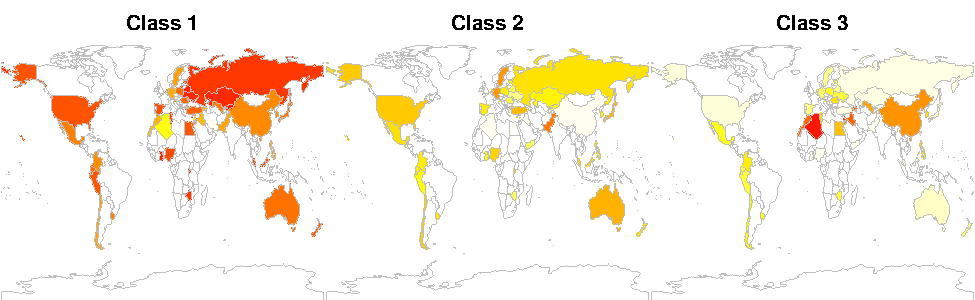
\includegraphics[width=\textwidth]{figures/maps.pdf}
	
	\caption{\label{fig:maps}}
\end{figure}

\begin{figure}
	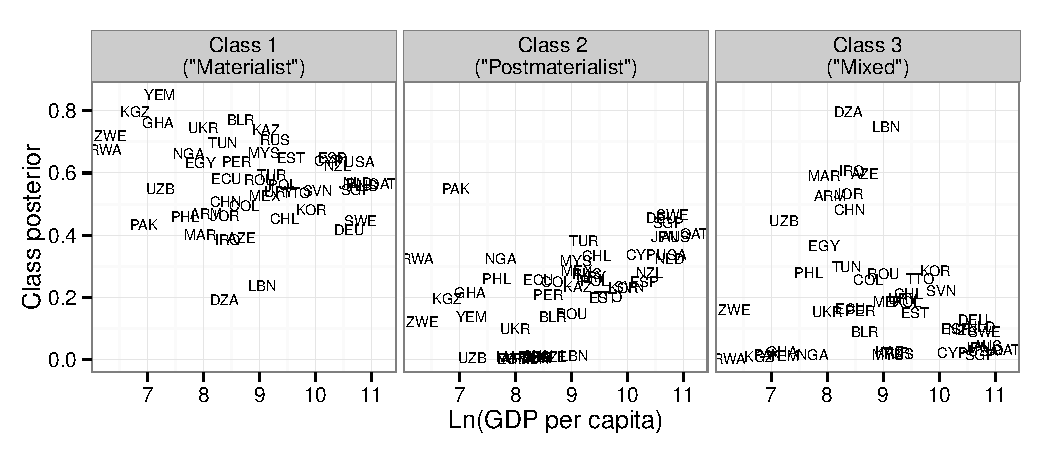
\includegraphics[width=\textwidth]{figures/gdp-posterior.pdf}
	
	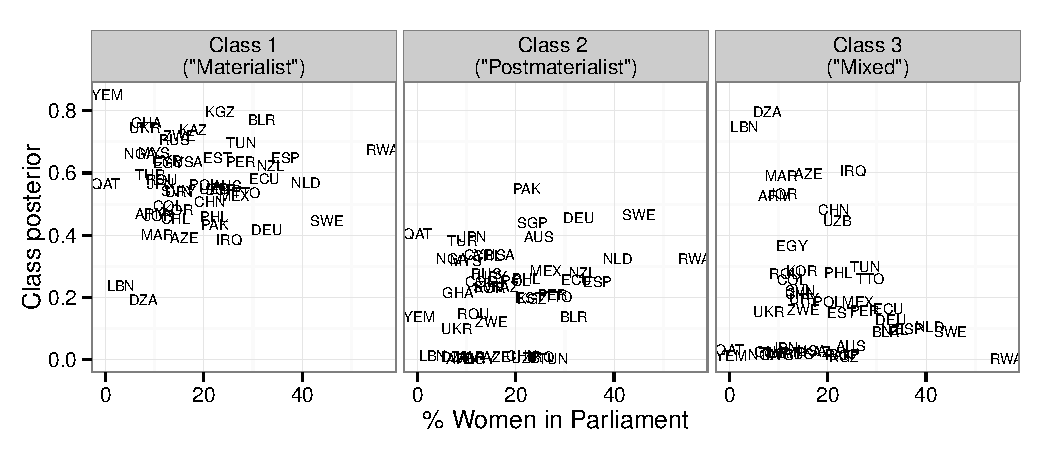
\includegraphics[width=\textwidth]{figures/women-posterior.pdf}

	\caption{\label{fig:posterior}}
\end{figure}
\fi


\begin{figure}
	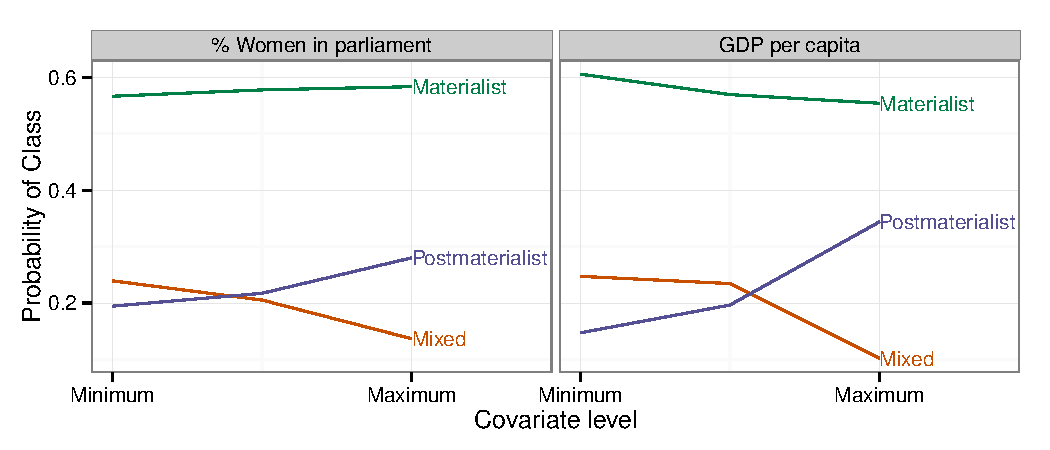
\includegraphics[width=\textwidth]{figures/covariates.pdf}
	\caption{\label{fig:covariates}Estimated probability of choosing each class as a function of the covariates of interest under the final model.}
\end{figure}

Finally, Figure \ref{fig:covariates} summarizes the loglinear parameter estimates of interest shown column 3 of Table \ref{tab:epc-interest-model2}. These graphs plot the covariate level on the horizontal axes and the probability of belonging to each of the classes defined in Table \ref{tab:attribute-parameters} on the vertical axes. The left-hand plot in Figure \ref{fig:covariates} shows the estimated marginal relationship between the percentage of women in parliament and the (post)materialism classes. It can be seen that the probability of the ``post materialist'' class is much larger for countries with a large percentage of women in parliament than it is for countries for fewer female parliamentarians: the predicted probability of belonging to the postmaterialist class for countries with the observed maximum percentage of women in parliament is 0.30, which is 7 percentage points above the average ``postmaterialist'' class membership of 0.23 (shown in Table \ref{tab:attribute-parameters}). The probability of belonging to the purely economical ``materialist'' class also increases very slightly, to the overall detriment of membership of the ``mixed'' class in which ``order in the nation'' and ``fighting crime'' is sometimes endorsed. 

The right-hand side of Figure \ref{fig:covariates} plots the estimated effect of log-GDP per capita on the three class membership probabilities. A similar pattern to that for percentage of women in parliament is observed for the ``postmaterialist'' and ``mixed'' classes, while the probability of belonging to the ``materialist'' class decreases somewhat with GDP per capita. The differences in predicted class membership are even larger over the observed GDP range than for the percentage of women in parliament: the predicted postmaterialist class membership at the maximum observed GDP is 0.40, which is 17 percentage points above the average. Greater prosperity is thus clearly strongly associated with postmaterialism. Crucially, the application of $\da{}$ leads to greater confidence that this conclusion is not an artefact of differences in measurement.




\section{Discussion and conclusion}
\label{sec:discussion}

Whenever groups are compared, measurement equivalence is a concern. Particularly, it should be verified that substantive conclusions of interest are uncontaminated by possible cross-group differences in measurement. The $\da$, a measure introduced by \citet{Oberski:WP:EPC-interest} for this purpose in the context of linear structural equation models, was extended in this paper to apply to categorical observed and latent variables as well as rankings and other types of data often encountered in the social sciences. An example application looked at the relationship between latent (post)materialism on the one hand and, on the other, log-GDP per capita and the percentage of women in parliament using data from  67,568 respondents in 48 countries. The $\da{}$ is a useful guide for this purpose, reducing a potentially 5076-dimensional problem to the examination of Tables \ref{tab:epc-interest-model1} and \ref{tab:epc-interest-model2}. Finally, we provided user-friendly  software implementing the $\da$; program input and data for the example application is available in the online Appendix. 

The EPC-interest fits within the recent literature on ``approximate measurement invariance''. That is, the goal of incorporating important measurement differences in the model while ignoring unimportant ones. Invariance testing using ``approximate'' fit measures such as the CFI and RMSEA \citep[e.g.][]{cheung2002evaluating,chen2007sensitivity} can be thought of as such a method, since the fit of the model is thought to be ``approximate'', and relative to model complexity. Model-based approaches include random effects modeling \citep{dejong2007relaxing,verhagen2013bayesian,jak2013test,jak2014measurement}, Bayesian priors on measurement differences \citep{muthen2012bayesian}, and factor rotation towards an invariant solution \citep{muthen2014alignment}. An advantage of these last three approaches is that a middle ground may be found between exact equality of measurement processes over groups and complete independence \citep{schoot2013facing}. However, a current problem  is that there is no agreed-upon definition of ``approximate''. At the same time, the EPC-interest approach does not offer a middle ground, but it does solve the problem of defining what ``approximate'' fit might be \citep[p. 12]{schoot2013facing}: for example, in the current application it was taken to be any measurement difference that cannot reverse the sign of the regression parameters of substantive interest.  An interesting direction for future work is therefore to combine the sensitivity analysis approach of the EPC-interest with the approaches to approximate measurement invariance of \citet{muthen2012bayesian,muthen2014alignment}, for example by weighting the cross-group measurement differences to be aligned by the possible change in parameters of interest. 

The scope of the paper was limited to an application of the EPC-interest to a model with categorical observed and latent variables. While we consider this a useful contribution, we did not further investigate the performance of this measure. We do note that the actually observed change in the parameters of interest after freeing the suggested invariance restrictions was very close to that predicted by the EPC-interest in this particular application. The Monte Carlo simulation using linear structural equation models  in \citet{Oberski:WP:EPC-interest} demonstrates that this is the case for linear structural equation models with relatively simple setups. However, an  investigation of whether this is the case for categorical latent class models under a wider range of hypothetical conditions in a simulation study remains work for the future.

%Dat jouw EPC-interest procedure een stap voorwaarts is, is zeer duidelijk. Dat je in dit empirisch voorbeeld sluitende resultaten hebt is veel minder en naar mijn aanvoelen te veel het gevolg van arbitraire keuzes die je hebt moeten maken in termen van het aantal latente klassen. Ik denk dat het verstandig is om aan de lezer alvast mee te geven dat het empirisch voorbeeld een illustratie is en niet een ?indepth? onderzoek naar de meetinvariante van het postmaterialisme meetinstrument.

\bibliographystyle{pa}
\bibliography{/Users/daob/Dropbox/Bibliography/quality}

\clearpage\appendix

\section{Countries included in the study}
\label{sec:countries-included}
\singlespacing
\begin{tabular}{lllll}
\hline
ISO3 code & Country name&&ISO3 code & Country name\\
\hline
DZA&	Algeria		&&MAR&	Morocco		\\
ARM&	Armenia		&&NLD&	Netherlands, The		\\
AUS&	Australia	&&NZL&	New Zealand		\\
AZE&	Azerbaijan	&&NGA&	Nigeria		\\
BLR&	Belarus		&&PAK&	Pakistan		\\
CHL&	Chile		&&PER&	Peru		\\
CHN&	China		&&PHL&	Philippines		\\
COL&	Colombia	&&POL&	Poland		\\
CYP&	Cyprus		&&QAT&	Qatar		\\
ECU&	Ecuador		&&RUS&	Russian Federation	\\
EGY&	Egypt		&&RWA&	Rwanda		\\
EST&	Estonia		&&SGP&	Singapore			\\
DEU&	Germany		&&SVN&	Slovenia		\\
GHA&	Ghana		&&ESP&	Spain		\\
IRQ&	Iraq		&&SWE&	Sweden		\\
JPN&	Japan		&&TTO&	Trinidad and Tobago	\\
JOR&	Jordan		&&TUN&	Tunisia		\\
KAZ&	Kazakhstan	&&TUR&	Turkey			\\
KOR&	Korea, Republic of  &&UKR&	Ukraine		\\
KGZ&	Kyrgyzstan	&&USA&	United States		\\
LBN&	Lebanon		&&URY&	Uruguay		\\
LBY&	Libya		&&UZB&	Uzbekista�		\\
MYS&	Malaysia        &&YEM&	Yemen		\\
MEX&	Mexico          &&ZWE&	Zimbabwe		\\	
\hline
\end{tabular}
\doublespacing

\clearpage
\section{Latent Gold Choice input for the full invariance model}\label{sec:LGinput}

The input below fits the full invariance model described in the paper, setting the possible violations of invariance to zero (0). The option ``score test'' in the output section (only available in Latent Gold or Latent Gold Choice $\geq5$) is then used to obtain the EPC-interest values.
Output and data for this example can be obtained from the online appendix at \url{http://}.

\begin{small}
\singlespace
\begin{verbatim}
options

   maxthreads=all;
   algorithm 
      tolerance=1e-008 emtolerance=0.01 
      emiterations=450 nriterations=70 ;
   startvalues
      seed=0 sets=30 tolerance=1e-005 iterations=50;
   bayes
      categorical=0 variances=0 latent=0 poisson=0;
   missing  excludeall;
   
   // NOTE: The option "scoretest" for output is used to obtain 
   //        the EPC-interest. This will also produce the score test ("MI")
   //        and EPC-self for the measurement invariance restriction
   
   output      
      parameters=effect  betaopts=wl standarderrors profile 
      probmeans=posterior
      frequencies bivariateresiduals estimatedvalues=regression
      predictionstatistics setprofile setprobmeans 
      iterationdetails scoretest ;

    // There are several ways of modeling ranking data using LG or LGChoice.
    //    The most computationally efficient is to use the so-called "3-file"
    //    setup in LGChoice employed here (see LGChoice manual). 

	choice = 3
   alternatives 'inglehart_wvs6_long.alt' quote = single
   id=alt
   choicesets 'inglehart_wvs6_long.set' quote = single
   id=set;

variables
   groupid country;
   caseid id;
   choicesetid set ;
   dependent value ranking;
   independent NY_GDP_PCAP_CD, SG_GEN_PARL_ZS;
   attribute int1 nominal, int2 nominal, int3 nominal;
   latent
      GClass  group nominal 3, 
      Class nominal 3;

equations
   // Group class intercept
   GClass <- 1 ;
   
   // Parameters of interest are logistic regression coefficients of 
   //        NY_GDP_PCAP_CD and SG_GEN_PARL_ZS.
   Class <- 1 + GClass + NY_GDP_PCAP_CD + SG_GEN_PARL_ZS;
   
   // Below, sets of possible violations of measurement invariance have been
   //        explicitly restricted to equal zero using "(0)". This will
   //        produce EPC-interest, EPC-self, and Score test output.
   value <- int1 + int2 + int3 + 
      int1 Class + int2 Class + int3 Class + 
      (0) int1 GClass + (0) int2 GClass + (0) int3 GClass + 
      (0) int1 Class  GClass + 
      (0) int2 Class GClass + 
      (0) int3 Class GClass ;
\end{verbatim}

\end{small}
\doublespacing

\clearpage
\section{Model selection for the example application}

\label{app:bic}

\begin{table}
\centering
\caption{Log-likelihood, number of parameters, and Bayesian Information Criterion (BIC) for models with different numbers of classes for the (post)materialism (within-country) and country group (between-country) latent class variables.\label{tab:loglikelihood-models}}
\begin{tabular}{rrrrrrrrr}
  \hline
 \multicolumn{4}{c}{(Post)materialism ($X$) classes, $|\{G\}| = 1$ } &  & \multicolumn{4}{c}{Country group ($G$) classes, $|\{X\}| = 3$} \\ 
\cline{1-4}\cline{6-9}
 \#Classes & Log-lik & \#Par & BIC($L^2$) &  & \#Classes & Log-lik & \#Par & BIC \\ 
  \hline
 1 & -460512.7 & 9 & -10346.1 &  & 1 & -447646.2 & 29 & 895616.3 \\ 
 2 & -449836.9 & 19 & -31586.2 &  & 2 & -444754.8 & 32 & 889867.0 \\ 
 3 & -447646.2 & 29 & -35855.8 &  & 3 & -443216.6 & 35 & 886824.1 \\ 
 4 & -446211.1 & 39 & -38614.4 &  & 4 & -442734.2 & 38 & 885892.8 \\ 
 5 & -445246.3 & 49 & -40432.4 &  & 5 & -442436.5 & 41 & 885330.9 \\ 
 6 & -444776.4 & 59 & -41260.3 &  & 6 & -442110.5 & 44 & 884712.3 \\ 
 7 & -444384.0 & 69 & -41933.4 &  & 7 & -441946.2 & 47 & 884417.3 \\ 
% 8 & -443959.8 & 79 & -42670.2 &  &  &  &  &  \\ 
% 9 & -443746.9 & 89 & -42984.3 &  &  &  &  &  \\ 
% 10 & -443470.8 & 99 & -43424.9 &  &  &  &  &  \\ 
% 11 & -443299.3 & 109 & -43656.2 &  &  &  &  &  \\ 
% 12 & -443086.0 & 119 & -43971.0 &  &  &  &  &  \\ 
% 13 & -442944.1 & 129 & -44143.3 &  &  &  &  &  \\ 
% 14 & -442837.3 & 139 & -44245.2 &  &  &  &  &  \\ 
   \hline
\end{tabular}
\end{table}

In choosing the number of classes for the (post)materialism (within-country) and country group (between-country) latent class variables, we follow the advice of \citet{lukovciene2010simultaneous} to first fix the number of country-group classes to unity and choose a number of within-country classes, subsequently fixing the number of within-country classes to this chosen number and determining the number of country-group (between-country) classes. The left-hand side of Table \ref{tab:loglikelihood-models} shows the log-likelihoods, number of parameters and Bayesian Information Criterion (BIC) values based on the $L^2$ for the model with one country-group class and an increasing number of (post)materialism classes. It can be seen that the BIC, which penalizes model complexity, decreases with each additional latent (post)materialism class. In fact, the BIC does not stop decreasing even when incrementing the number of classes to 14 (not shown in Table \ref{tab:loglikelihood-models} for brevity). 

In the literature on (post)materialism \citep[e.g.][]{inglehart1997modernization,inglehart2002gender,inglehart2010changing}, the number of (post)materialism classes is typically fixed to three: ``postmaterialist'', ``materialist'', and ``mixed''. Clearly, using the WVS ranking tasks and imposing full invariance, many more qualitative (post)materialism classes can be distinguished than the traditional three classes. This corresponds to findings by \citet{moors2007heterogeneity}; however, these authors \citep[following][]{hagenaars1990categorical} also argued that ``one can safely interpret the results (...) if adding another class does not result in important changes of the latent class weights for the other classes'' (p. 637). While this is a somewhat subjective criterion, the three-class solution found in the data does correspond to  the theoretical ``postmaterialist'', ``materialist'', and ``mixed'' classes, whose  parameters appear to change little in the models with a greater number of classes. Moreover, the greatest reduction in BIC seen in Table \ref{tab:loglikelihood-models} takes place when moving from a one-class to a two-class model, with relatively small improvements after three or more classes. We therefore follow the theoretical literature in selecting the three-class model.

While selecting the number of country-group classes, we find that the BIC improves little after three classes (right-hand side of Table \ref{tab:loglikelihood-models}), so that our initial full invariance model has three (post)materialism (within-country) and three country group (between-country) classes. 



\if 1=2
\section{Derivatives for the  multilevel latent class model}
\label{app:derivatives}
\doublespacing
For the application involving categorical latent and observed variables, $\bpsi$  corresponds to the direct effects $\tau^*_{jkg}$ and $\lambda^*_{jkxg}$ in Equation \ref{eq:loglin-measurement-noninvariant} (see also Figure \ref{fig:model}). The Jacobian of the individual likelihood with respect to the $\tau^*_{jkg}$ parameters is 
\begin{equation}
	\frac{\partial L_i(\param) }{\partial \tau^*_{jkg}} = 
		L_i(\param) \sum_G \left[ P(G|) \sum_X P(X|Z_1, Z_2) ( Y_{jk}G_g - E[ Y_{jk}G_g | X]) \right],
		\label{eq:derivative-main}
\end{equation}
Similarly,
\begin{equation}
	\frac{\partial L_i(\param) }{\partial \lambda^*_{jkxg}} = 
		L_i(\param) \sum_G \left[ P(G) \sum_X P(X|Z_1, Z_2) ( Y_{jk} X_x G_g  - E[ Y_{jk} X_x G_g | X]) \right],
		\label{eq:derivative-interaction}
\end{equation}
where $X_x$ is the effect-coded value for class $x$ of the within-country latent (post)materialism variable $X$.  The derivatives for other parameters of the model are given by  \citet{vermunt2013technical}. These have a form similar to Equations \ref{eq:derivative-main} and \ref{eq:derivative-interaction}. Consistent estimates of all derivatives can be obtained by replacing the parameters of the model by their maximum likelihood estimates, providing the  vector $[ \left.\partial L(\param, \bpsi) / \partial \bpsi ] \right|_{\param = \that}$  necessary for calculating Equation \ref{eq:epc-interest}.



\fi
\end{document}
